\subsection{Related work}
This section discusses earlier created software projects that have attempted to solve the described problem or offer solutions for parts of the problem.

\subsubsection*{$\bullet$ pyLOB}
PyLOB \cite{pyLOB} is an open source project that simulates a financial exchange.
It does this by keeping an orderbook that contains all previously made bids and asks.
Whenever two offers match, it automatically simulates a trade and removes the offers from the orderbook.
While PyLOB is not decentralised, the simulation helps to understand how bids, asks, and matching trades work.
It also contained a large dataset of offers from a real exchange, which can be used in different simulations.

\subsubsection*{$\bullet$ BarterCast}
BarterCast \cite{bartercast} is a fully distributed system that manages reputation of peers among a network. 
It uses the epidemic protocol, also called gossip protocol, to spread information about the amount of data uploaded and downloaded by every peer.
Users uploading data use this information to decide who gets priority on receiving files.
Peers that have a better reputation of uploading get more slots to download from, since more peers are willing to share their data with them.
We used the same epidemic communication protocol in Tsukiji as scalable messaging solution.\\

The following projects were found later in the development and their ideas did not influence Tsukiji's development process.
They are nonetheless closely related projects and are worth mentioning.

\subsubsection*{$\bullet$ Bitmarkets}
Bitmarkets\cite{bitmarkets} is a free OSX application for a decentralised marketplace.
Users communicate using Bitmessage \cite{bitmessage} to hide the identity of the creator of a message.
These messages are sent to other users via the Tor \cite{tor} network.
This way both the identity and location of the originator are hidden.
The only thing visible is a public key generated by Bitmessage that can be used to reply to.
Payments are done using BitCoin's multi-signature transactions.
This requires both parties to sign a transaction before the BitCoins are moved from wallet to wallet.

\subsubsection*{$\bullet$ OpenMarket}
OpenMarket \cite{openmarket} is another BitCoin-based decentralized market.
Rather than one large marketplace of buyers and sellers, OpenMarket lets people set up their own webshop.
This locally hosted website supports all functionality one would expect of a webshop.
Items to be sold can be added to the store with images and prices. 
Potential buyers can go to this site and browse the catalog of this particular seller.
Whenever a buyer wants to buy an item, they can add the item to a shopping cart and can checkout the whole cart.
Payment is handled by the BitCoin network.
\begin{figure}[H]
  \centering
  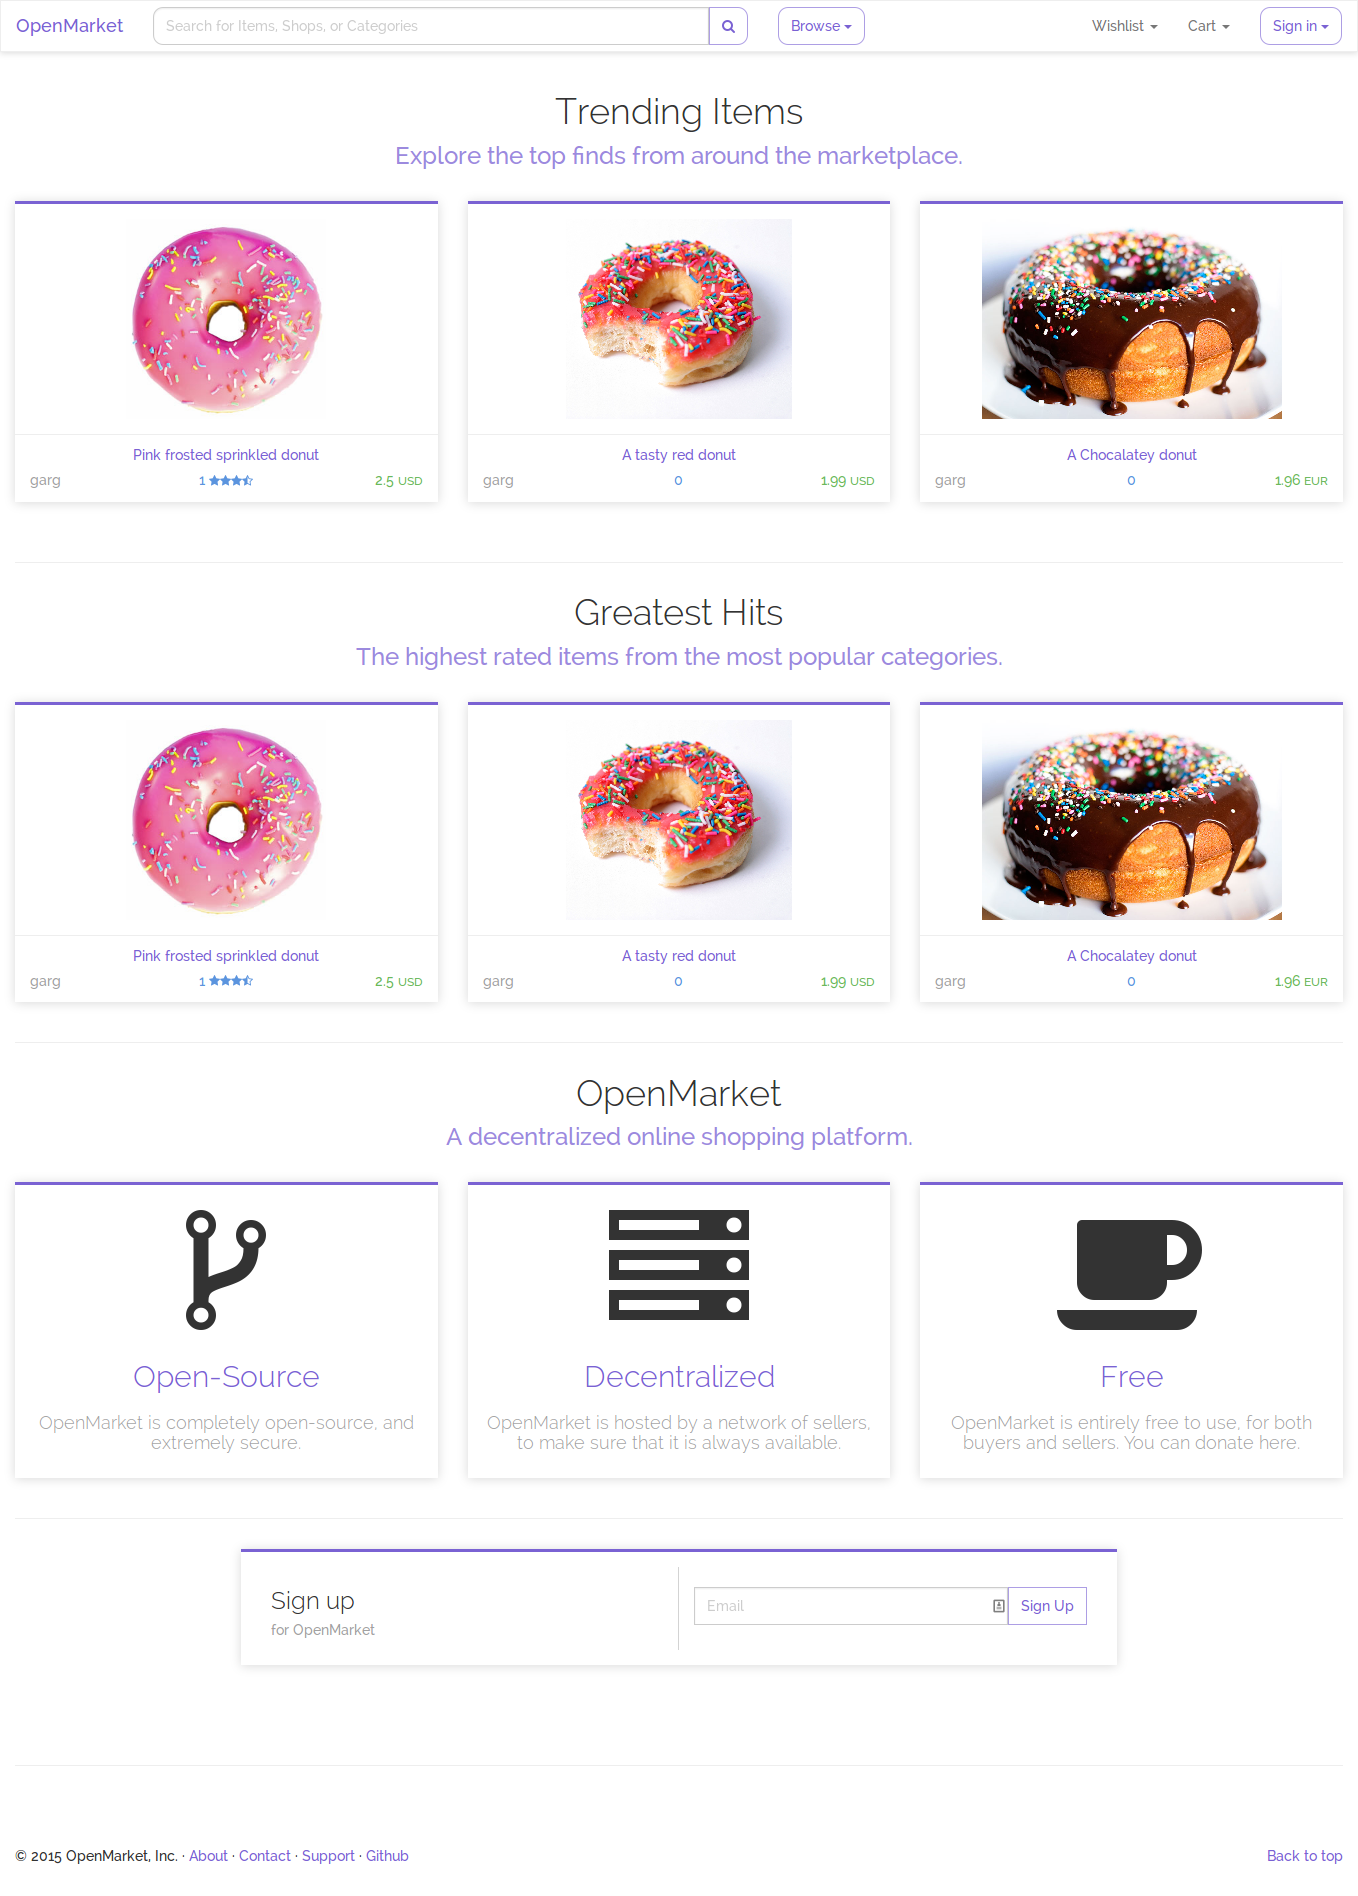
\includegraphics[scale=0.2]{openmarket}
  \caption{Example of a webstore created by OpenMarket\cite{opemarketpic}}
  \label{openmarketfig}
\end{figure}
The difference between Tsukiji and OpenMarket is that OpenMarket is not one large marketplace.
It is a lot of small markets that have no knowledge of each other.
There is no network of markets, just a large amount of separate ones.

\subsubsection*{$\bullet$ OpenBazaar}
OpenBazaar \cite{bazaar} is also a decentralised marketplace where goods are traded with BitCoin.
It uses a Distributed Hash Table to connect peers to each other in a scalable way.
The software opens a webpage that represents the bazaar and users can create their own shops on the bazaar.
Users can visit other shops and buy items from them, or simply wait until items are bought from their own shop.
Items being sold are hashed and this hash is used to create a contract.
Whenever someone buys an item, they sign the contract and send it to the seller.
The seller then sends it to an independent third person, or escrow, on the network.
This escrow signs the contract and the buyer sends bitcoin to a multisig deposit that can only be opened by at least two of the three keys.
Any conflicts between the two parties (e.g., one side did not receive their goods) are resolved by an independent arbiter \cite{bazaarDisputeResolution}.
While this is a great structure to reduce trust issues between parties, it is reliant on BitCoin.
Not all forms of currency are as easily locked away and retrieved.